\documentclass[8pt,a4paper]{article} % Compila con lualatex o xelatex

% --- Layout & links ---
\usepackage[margin=1.5in]{geometry}
\usepackage[hidelinks]{hyperref}

% --- Fuentes (texto y matemáticas) ---
\usepackage{newtxmath}
\usepackage{fontspec}
% \setmainfont{EB Garamond}[
%   UprightFont = * Medium,
%   ItalicFont = * Medium Italic,
%   BoldFont = * SemiBold,
%   BoldItalicFont = * SemiBold Italic
% ]
\setmainfont{EB Garamond}[
  UprightFont = * Regular,
  ItalicFont = * Italic,
  BoldFont = * SemiBold,
  BoldItalicFont = * SemiBold Italic
]

% --- Secciones y subsecciones ---
\usepackage{titlesec}
\newfontface\garamondbold{EB Garamond SemiBold}
\newfontface\garamondbolditalic{EB Garamond SemiBold Italic}
\titleformat{\section}
  {\garamondbold\Large}{\thesection}{1em}{}
\titleformat{\subsection}
  {\garamondbold\Large}{\thesubsection}{1em}{}

% --- Encabezado con nombre de la sección ---
\usepackage{fancyhdr}
\pagestyle{fancy}
\fancyhf{}
\fancyhead[L]{\small\leftmark}
\fancyhead[R]{\small\thepage}
\renewcommand{\headrulewidth}{0.0pt}

% --- Espaciado ---
\usepackage{setspace}

% --- Otros paquetes útiles ---
\usepackage{tocloft}  % Para personalizar la tabla de contenidos
\usepackage{xcolor}   % Para colores en el código
\usepackage{booktabs} % Para tablas bonitas
\usepackage{graphicx} % Para las graficas
\graphicspath{{../../../../visualizations/figuras/}}


% --- Código fuente ---
\usepackage{listings}
\lstset{
  basicstyle=\ttfamily\small,
  backgroundcolor=\color{gray!10},
  frame=single,
  breaklines=true
}


\usepackage{chngcntr}       % in preamble
\numberwithin{figure}{subsection}


\usepackage{lipsum}

\begin{document}

% --- Portada ---
\begin{titlepage}
  \centering
  \vspace*{4cm}
  {\Huge\bfseries CMAT\par}
  \vspace{2cm}
  {\Large Author Name\par}
  \vspace{1cm}
  {\large Universidad de las Américas Puebla\par}
  \vfill
  {\large \today\par}
\end{titlepage}

% --- Abstract ---
\begin{abstract}
This document provides a template for reports in the "AI in Financial Services" course, using EB Garamond for prose and Libertinus Math for formulas. It includes a cover page, abstract, table of contents, and sample sections for math and text. Additional content demonstrates tables, code, and references.
\end{abstract}

% --- Tabla de contenidos ---
\tableofcontents
\thispagestyle{empty}
\newpage

% --- Inicio del documento ---
\section{Overview}
This document is a minimal example using EB Garamond for prose and libertinust1math for formulas.
Links like \href{https://example.com}{this one} are active.


\newpage
\section{What is CMAT?}
Centro de Matematicas, (Math Center), is a place where students go to take assesorias.



\newpage
\section{Exploratory Data Analysis}
\lipsum[1]

\subsection{How many people went to CMAT?}
\lipsum[1]

\begin{figure}[h]
    \centering
    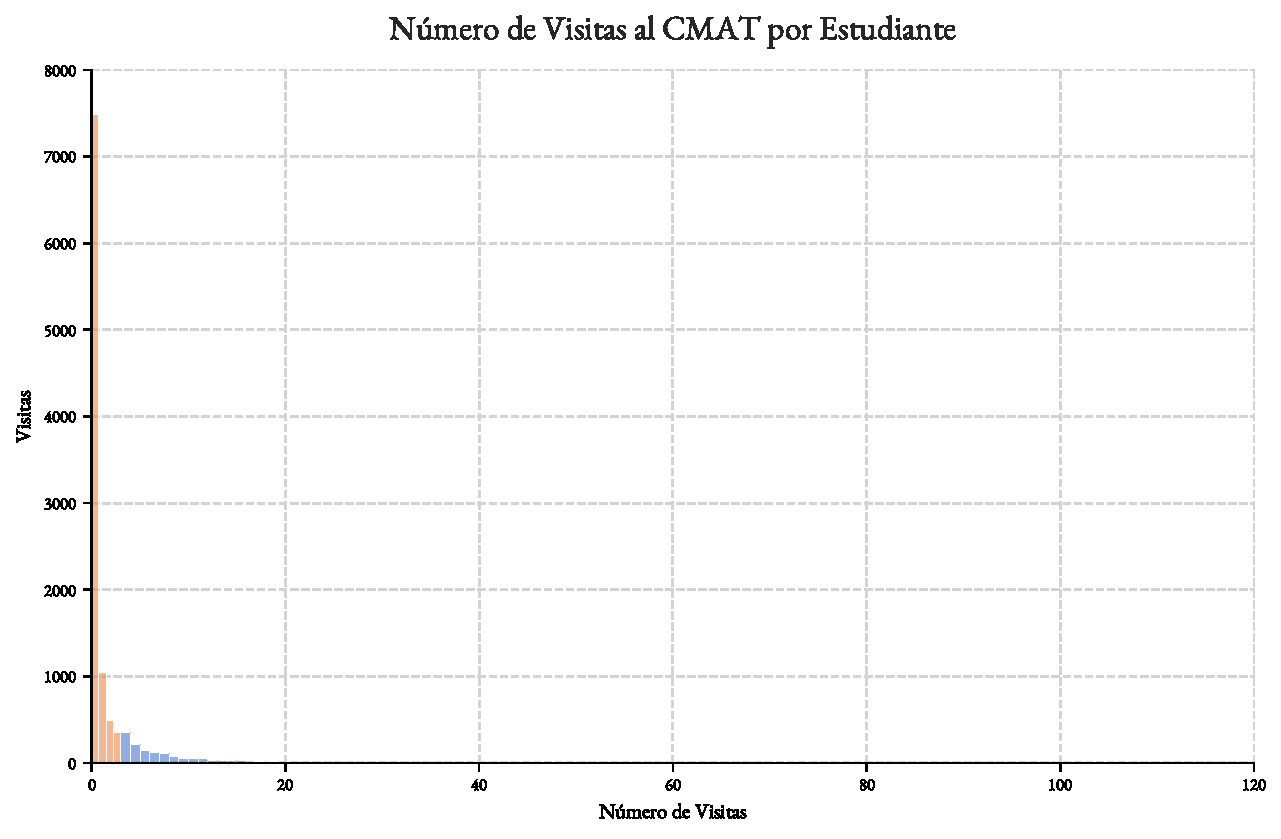
\includegraphics[width=0.7\textwidth,page=1]{03_01.pdf}
    \caption{PDF imported as image}
\end{figure}

\end{document}